\documentclass[letta4 paper]{article}
% Set target color model to RGB
\usepackage[inner=2.0cm,outer=2.0cm,top=2.5cm,bottom=2.5cm]{geometry}
\usepackage{setspace}
\usepackage[rgb]{xcolor}
\usepackage{verbatim}
\usepackage{subcaption}
\usepackage{amsgen}
\usepackage{amsmath}
\usepackage{amstext}
\usepackage{amsbsy}
\usepackage{amsopn}
\usepackage{tkz-linknodes}
\usepackage{fancyhdr}
\usepackage[colorlinks=true, urlcolor=blue,  linkcolor=blue, citecolor=blue]{hyperref}
\usepackage[colorinlistoftodos]{todonotes}
\usepackage{rotating}
\usepackage{listings}
\usepackage{algorithm}
\usepackage{algorithmic}
\usepackage{fancyhdr}
\usepackage{enumitem}
\usepackage{gensymb}
\usepackage{siunitx}
\usepackage{tikz}
\usepackage[T1]{fontenc}
\usepackage[thinlines]{easytable}
\usepackage{subcaption}
\lstset{
%	language=bash,
	basicstyle=\ttfamily,
    breaklines=true,
    postbreak=\mbox{$\hookrightarrow$\space},
}

\newcommand{\lvanumber}{182.731}
\newcommand{\lvasemester}{2022S}
\newcommand{\lvainfo}{(VU 4,0)}
\newcommand{\lvaname}{GPU Architectures and Computing}
\newcommand{\labname}{Project: Find connected components in an undirected graph}

\newcommand{\labstartdate}{\today}
\newcommand{\labenddate}{\today}

\newcommand{\ra}[1]{\renewcommand{\arraystretch}{#1}}

\newtheorem{thm}{Theorem}[section]
\newtheorem{prop}[thm]{Proposition}
\newtheorem{lem}[thm]{Lemma}
\newtheorem{cor}[thm]{Corollary}
\newtheorem{defn}[thm]{Definition}
\newtheorem{rem}[thm]{Remark}
\numberwithin{equation}{section}
\graphicspath{ {./img/} }

\pagestyle{fancy}
\fancyhf{}
\lhead{\lvaname~\lvasemester}
\rhead{\labname}
\cfoot{Page \thepage}

\newcommand{\homework}[2]{
   \newpage
   \setcounter{page}{1}
   \noindent
   \begin{center}
   \framebox{
      \vbox{\vspace{2mm}
        \begin{minipage}{0.3\textwidth}
        
\includegraphics[width=\textwidth]{TU_logo.png}
        \end{minipage}
        ~
        \begin{minipage}{0.65\textwidth}
        \centering
        \normalsize \bf \lvaname \\ \lvanumber~\lvainfo~Semester: \lvasemester \\
        \vspace{2mm}
        \Large {#1}\\
        \vspace{2mm}
        \normalsize \bf #2
        \end{minipage}
      \vspace{2mm}}
   }
   \end{center}
   \vspace*{4mm}
}

\newcommand{\simpletodo}[1]{\textcolor{red}{\textbf{TODO:} #1}}

\newcommand{\problem}[3]{~\\\fbox{\textbf{Problem #1: #2}}\hfill (#3 points)\newline}
\newcommand{\subproblem}[1]{~\newline\textbf{(#1)}}
\newcommand{\D}{\mathcal{D}}
\newcommand{\Hy}{\mathcal{H}}
\newcommand{\VS}{\textrm{VS}}
\newcommand{\solution}{~\newline\textbf{\textit{(Solution)}} }

\newcommand{\bbF}{\mathbb{F}}
\newcommand{\bbX}{\mathbb{X}}
\newcommand{\bI}{\mathbf{I}}
\newcommand{\bX}{\mathbf{X}}
\newcommand{\bY}{\mathbf{Y}}
\newcommand{\bepsilon}{\boldsymbol{\epsilon}}
\newcommand{\balpha}{\boldsymbol{\alpha}}
\newcommand{\bbeta}{\boldsymbol{\beta}}
\newcommand{\0}{\mathbf{0}}

\usepackage{booktabs}



\begin{document}

	\homework {\labname}{\labstartdate}
	\thispagestyle{empty}

	\section*{Student data}

\noindent
\begin{tabular}{| l | l | l|} 
 \hline
 \textbf{Matrikelnummer} & \textbf{Firstname} & \textbf{Lastname} \\
 \hline
 01525189 & Christoph & Lehr  \\
 \hline
 11810276 & Manuel & Reinsperger \\
 \hline
 11809637 & Lukas & Rysavy \\
 \hline
\end{tabular}

\section{Problem statement}
The goal of this project is, given an undirected graph, to find a list of connected components in said graph, ie. maximal sets of nodes connected to each other. Input graphs are weighted, but only the fact whether two nodes are connected is relevant for the task, and path costs can be ignored.

\newpage

\section{Input data format}
Graphs are supplied in input files with the following format: The first line has the format \texttt{H <n> <e> <u>}, with the number of nodes \texttt{<n>}, number of edges \texttt{<e>} and whether the graph is undirected (\texttt{<u>}, always 1). This line is followed by \texttt{<e>} lines, each describing an edge \texttt{E <s> <d> <w>} with source node \texttt{<s>}, destination node \texttt{<d>} and weight \texttt{<w>} (irrelevant), where nodes are numbered from 0 to \texttt{<n>}-1.

\section{Building and Running}

In each project directory a \texttt{Makefile} is located which builds each implementation when executing \texttt{make} as a \texttt{connected\_components} binary. Each implementation has 4 modes of operation:
\begin{itemize}
    \item \texttt{generate}: Generates a graph
        \begin{itemize}
            \item \texttt{filename}: Path where the generated graph shall be stored
            \item \texttt{nodes}: The number of nodes that shall be in the generated graph
            \item \texttt{density}: How densely connected the graph shall be, with 0 for no connections and 1 for all nodes connected to all other nodes
            \item \texttt{min\_weight}: Minimum weight of an edge
            \item \texttt{max\_weight}: Maximum weight of an edge
        \end{itemize}
    \item \texttt{bench}: Runs the implementations internal benchmarks
        \begin{itemize}
            \item \texttt{rounds}: How many round shall be executed
            \item \texttt{nodes}: How many nodes shall be generated for the bench-marking graph
            \item \texttt{do-checking}: Set to \texttt{1} if the results shall be checked to be equal.
        \end{itemize}
    \item \texttt{calculate}: Calculates the connected components with a given algorithm 
        \begin{itemize}
            \item \texttt{impl}: Which implementation to run
            \item \texttt{filename}: Which input file shall be used
            \item \texttt{--generate}: Indicates a graph shall be generated instead of using an input file
                \begin{itemize}
                    \item \texttt{nodes}: The number of nodes that shall be in the generated graph
                    \item \texttt{density}: How densely connected the graph shall be, with 0 for no connections and 1 for all nodes connected to all other nodes
            \end{itemize}
        \end{itemize}
    \item \texttt{evaluate}: Runs the evaluation test suite
        \begin{itemize}
            \item \texttt{folder}: The folder which shall be used as an input for the evaluation
        \end{itemize}
\end{itemize}

\subsection{Implementation Selection}

Each algorithm has various implementations to select, with the ids listed below:
\begin{itemize}
    \item Sparse Representation - one thread per Connected component
        \begin{enumerate}[label=\arabic*]\addtocounter{enumi}{-1}
            \item CPU implementation
            \item GPU implementation 
            \item GPU implementation with vector as output
            \item GPU implementation using pinned memory
            \item GPU implementation using pinned memory with vector as output
            \item GPU implementation using zero-copy memory
            \item GPU implementation using zero-copy memory with vector as output
        \end{enumerate}
    \item Dense Matrix Representation
        \begin{enumerate}[label=\arabic*]\addtocounter{enumi}{-1}
            \item CPU implementation
            \item GPU implementation
            \item GPU implementation using pinned memory
            \item GPU implementation using zero-copy memory
        \end{enumerate}
    \item Thrust: consists only of the thrust implementation
\end{itemize}

\subsection{Evaluation}

The files generated to evaluate the algorithms are to large to add them to repository/handin. Therefore, the files are stored inside the \texttt{evaluate} folder insider our user home directory.

\newpage

\section{Implementations}
Throughout the project, we have developed a few different implementations, all
fulfilling the common goal of finding connected components in a graph. These
implementations differ in the algorithm used, input and output data formats,
and, on a more fine-grained level, the way of transferring memory between the
host system and the GPU.

Each subsection of this section will focus on one
of these implementations, comparing different variants within their
scopes. Section \ref{sec:compare} will compare the implementations to each
other.

\subsection{Sparse graph representation - thread per CC}
\subsubsection{Input format}
In this implementation, input is represented in a format especially suitable
for sparse graphs: A list of nodes is saved, each entry containing a pointer
to a list of node indices it is directly connected to. These edge lists can be
located directly after one another in memory, resulting in one large list and
pointers to somewhere in the middle of this list to allow for a very compact
structure.

\subsubsection{Algorithm}
The idea behind this version's algorithm is that every connected component is
"owned" by a single thread - the thread with the id of the highest node index
in the component. Each thread starts at its own node (the node with index =
thread id) and grows its own component by traversing the graph. If at some
point a thread realizes the component is owned by another thread (because it
encounters a node with an index greater than the start index), it
terminates. After a finite amount of steps (each thread traverses its
component or exits prematurely), a list of connected components is
returned.

Since the number of components is unknown in the beginning
(between 1 (all nodes connected) and n (no edges)), the number of threads must
be n (the number of nodes) in the beginning, and might shrink to any number
$\ge 1$. In this extreme case, the algorithm is completely sequential
(performed by the one surviving thread).

\subsubsection{Variants}
Using the same algorithm, we implemented two different versions: In one, each
thread gets space for their own component of at most n nodes, where it can
write results to. Threads that don't own a component simply set the number of
nodes of their component to zero. Of course, this means that $O(n^2)$ bytes
are required to store the output ($1-n$ components with $1-n$ nodes
each). However, this block of memory can be reused by the threads as a local
worklist.

The alternative version stores a single vector with one entry for each node
containing the id of the component it belongs to (two indices contain the same
id $\Leftrightarrow$ the two nodes belong to the same component). This only
needs $O(n)$ bytes of storage for the result, but a worklist of length n is
still needed for each thread, negating this advantage somewhat (however, a
list of booleans can be used, decreasing storage needed at least by a constant
factor). In addition, this approach requires the use of atomic operations
(updating the vector with an atomic `max` operation to ensure the component id
is the maximum index of its nodes), which can slow down the process if a lot
of conflicting accesses have to be made.

In addition, both of these approaches have been implemented using standard
memory transfer, pinned memory, and zero-copy memory.

\subsubsection{Results}
In general, the various implementations running on the GPU are faster than the
CPU for low graph densities. As the density increases, however, the CPU
version quickly overtakes all of them. Furthermore, the implementation storing
its outputs is even faster than the one giving each thread space to store a
component for low densities, but even slower for dense graphs. This can be seen in figure \ref{fig:sparse} for 1000 (\ref{fig:sparse1000}) and 10,000 (\ref{fig:sparse10000}) nodes.

\begin{figure}
    \centering
    \begin{subfigure}{0.45\textwidth}
        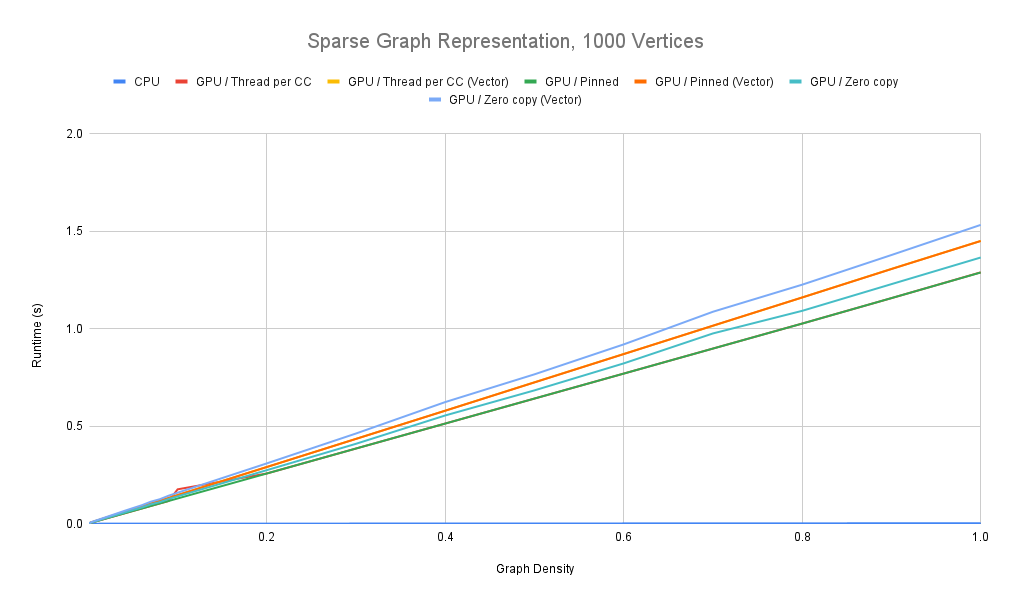
\includegraphics[width=\textwidth]{img/sparse/sparse1000.png}
        \caption{1000 Nodes}
        \label{fig:sparse1000}
    \end{subfigure}
    \hfill
    \begin{subfigure}{0.45\textwidth}
        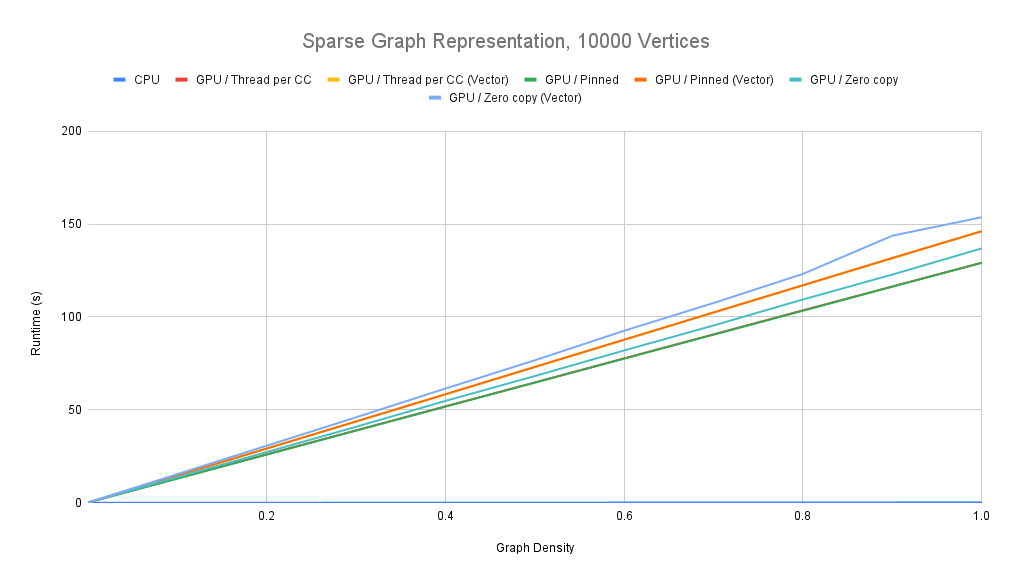
\includegraphics[width=\textwidth]{img/sparse/sparse10000.png}
        \caption{10000 Nodes}
        \label{fig:sparse10000}
    \end{subfigure}
    \caption{Comparison of algorithms}
    \label{fig:sparse}
\end{figure}

When using zero-copy memory, the algorithm takes more time than when device
memory is used by a factor proportional to the graph size (mainly number of
edges, which is also capped by the number of nodes); this can be seen in
figure \ref{fig:zerocopy_overhead}, with the number of nodes and graph density
on the horizontal axes (right/left respectively) and the overhead in seconds
on the vertical axis.

\begin{figure}
    \centering
    \includegraphics[width=.45\textwidth]{img/zerocopy.png}
    \caption{Overhead of zero-copy memory over device memory}
    \label{fig:zerocopy_overhead}
\end{figure}

Using pinned host memory naturally doesn't have any effect on the runtime of the algorithm itself, but it does decrease the time needed for memcpy operations to the device memory. This difference shows no clear pattern related to the graph size as can be seen in figure \ref{fig:pinned}, but is generally higher for larger graphs.

\begin{figure}
    \centering
    \includegraphics[width=.45\textwidth]{img/pinned.png}
    \caption{Speedup when using pinned memory}
    \label{fig:pinned}
\end{figure}

\subsubsection{Evaluation}
The difference between the performance of the GPU algorithms on sparse and on dense graphs can easily be explained: Dense graphs contain a low number of connected components, while in sparse graphs less nodes are connected and they thus contain more independent components (up to $n$ for a density of 0). If now each component is handled by exactly one thread, the number of effective threads shrinks relatively quickly as the density increases. In the worst case, the graph only contains a single component - here, all of the work is done by a single thread, and the algorithm is therefore completely sequential. Since a CPU thread greatly outperforms a single GPU thread, results are therefore bad in such cases.

The difference between the two output formats (vector and component list) can be explained with atomic operations: While the vector representation is much more compact and therefore fits into caches more easily (making this version faster for low densities), many threads access the same vector elements (nodes) if the graph is dense, leading to collisions of atomic operations and thus slowdowns.

The results on zero-copy memory also match expectations: Memory accesses take longer by a constant factor, and the amount of memory that needs to be accessed depends on the size of the graph. Therefore, the extra time needed grows proportionally with the graph size, which is exactly what can be observed.

Speedups when pinned memory is used are less consistent, but still match what is expected: The memcpy operation is slower when paging occurs, which happens more frequently for bigger quantities of data. Therefore, speedups are generally higher for larger graphs, because paging can be prevented more often, but there is still a random component involved.


\subsection{Dense graph representation}
\subsubsection{Input format} \label{dense_graph_input_format}

This implementation uses a dense format for data processing. This means that a full $n*n$ matrix is used, where $n$ is the number of nodes of the graph. It uses a lot more memory than the sparse format for graphs that are not too dense, but allows the algorithm to do column and row based matrix calculations.

\subsubsection{Algorithm}

This approach takes the given adjacency matrix and iterates over the single rows. The matrix is traversed row by row starting with index 0 or vertex 0 and skips entries which have already been assigned a connected component. When an entry is found, which does not belong to a connected component yet, all vertices which are connected to it are added to an array which holds all found nodes. Next, the algorithm starts iterating over this array and adds all vertices it finds to it. This is repeated until no further vertices are added to the array. Last but not least, each vertex gets assigned a connected component, where the id is the lowest found index.

The algorithm is implemented on the CPU by iterating over each row of the adjacency matrix, but on the GPU this process can be executed in parallel. For each node a thread shall be spawned, therefore a row of the matrix can be evaluated in constant time instead of iterating over $n$ iterations. 

\subsubsection{Results}

In Figure~\ref{fig:dense_matrix_impl_comparison} and Figure~\ref{fig:dense_matrix_memory_comparison} the run-time measurements of the algorithms using dense matrices are depicted. On the x-axis, the density of the graphs are depicted, and on the y-axis the run-time in seconds. All graphs used for the measurements have 10,000 vertices with various density.

What we can see in Figure~\ref{fig:dense_matrix_impl_comparison} is that run-time of the CPU algorithm grows linearly with the density of the graph, in contrast the GPU algorithm with parallel workflow which is mainly dependent on the size of the graph. 

in Figure~\ref{fig:dense_matrix_memory_comparison} a comparison of the same algorithm using normal GPU memory, pinned memory and zero-copy memory is shown. For the comparison the adjacency matrix, which is the basis on which the algorithm operates on, was stored in the different memory types. When looking at the diagram of Figure~\ref{fig:dense_matrix_memory_comparison}, execution times are quite similar. The access to the memory optimised to access one row at a time in parallel by all threads, this is optimizes the memory latency. As the host memory is significantly slower than the device memory, this points out that the limiting factor is the algorithm itself and not the memory interface.

\begin{figure}
    \centering
    \begin{minipage}{.5\textwidth}
    	\centering
    	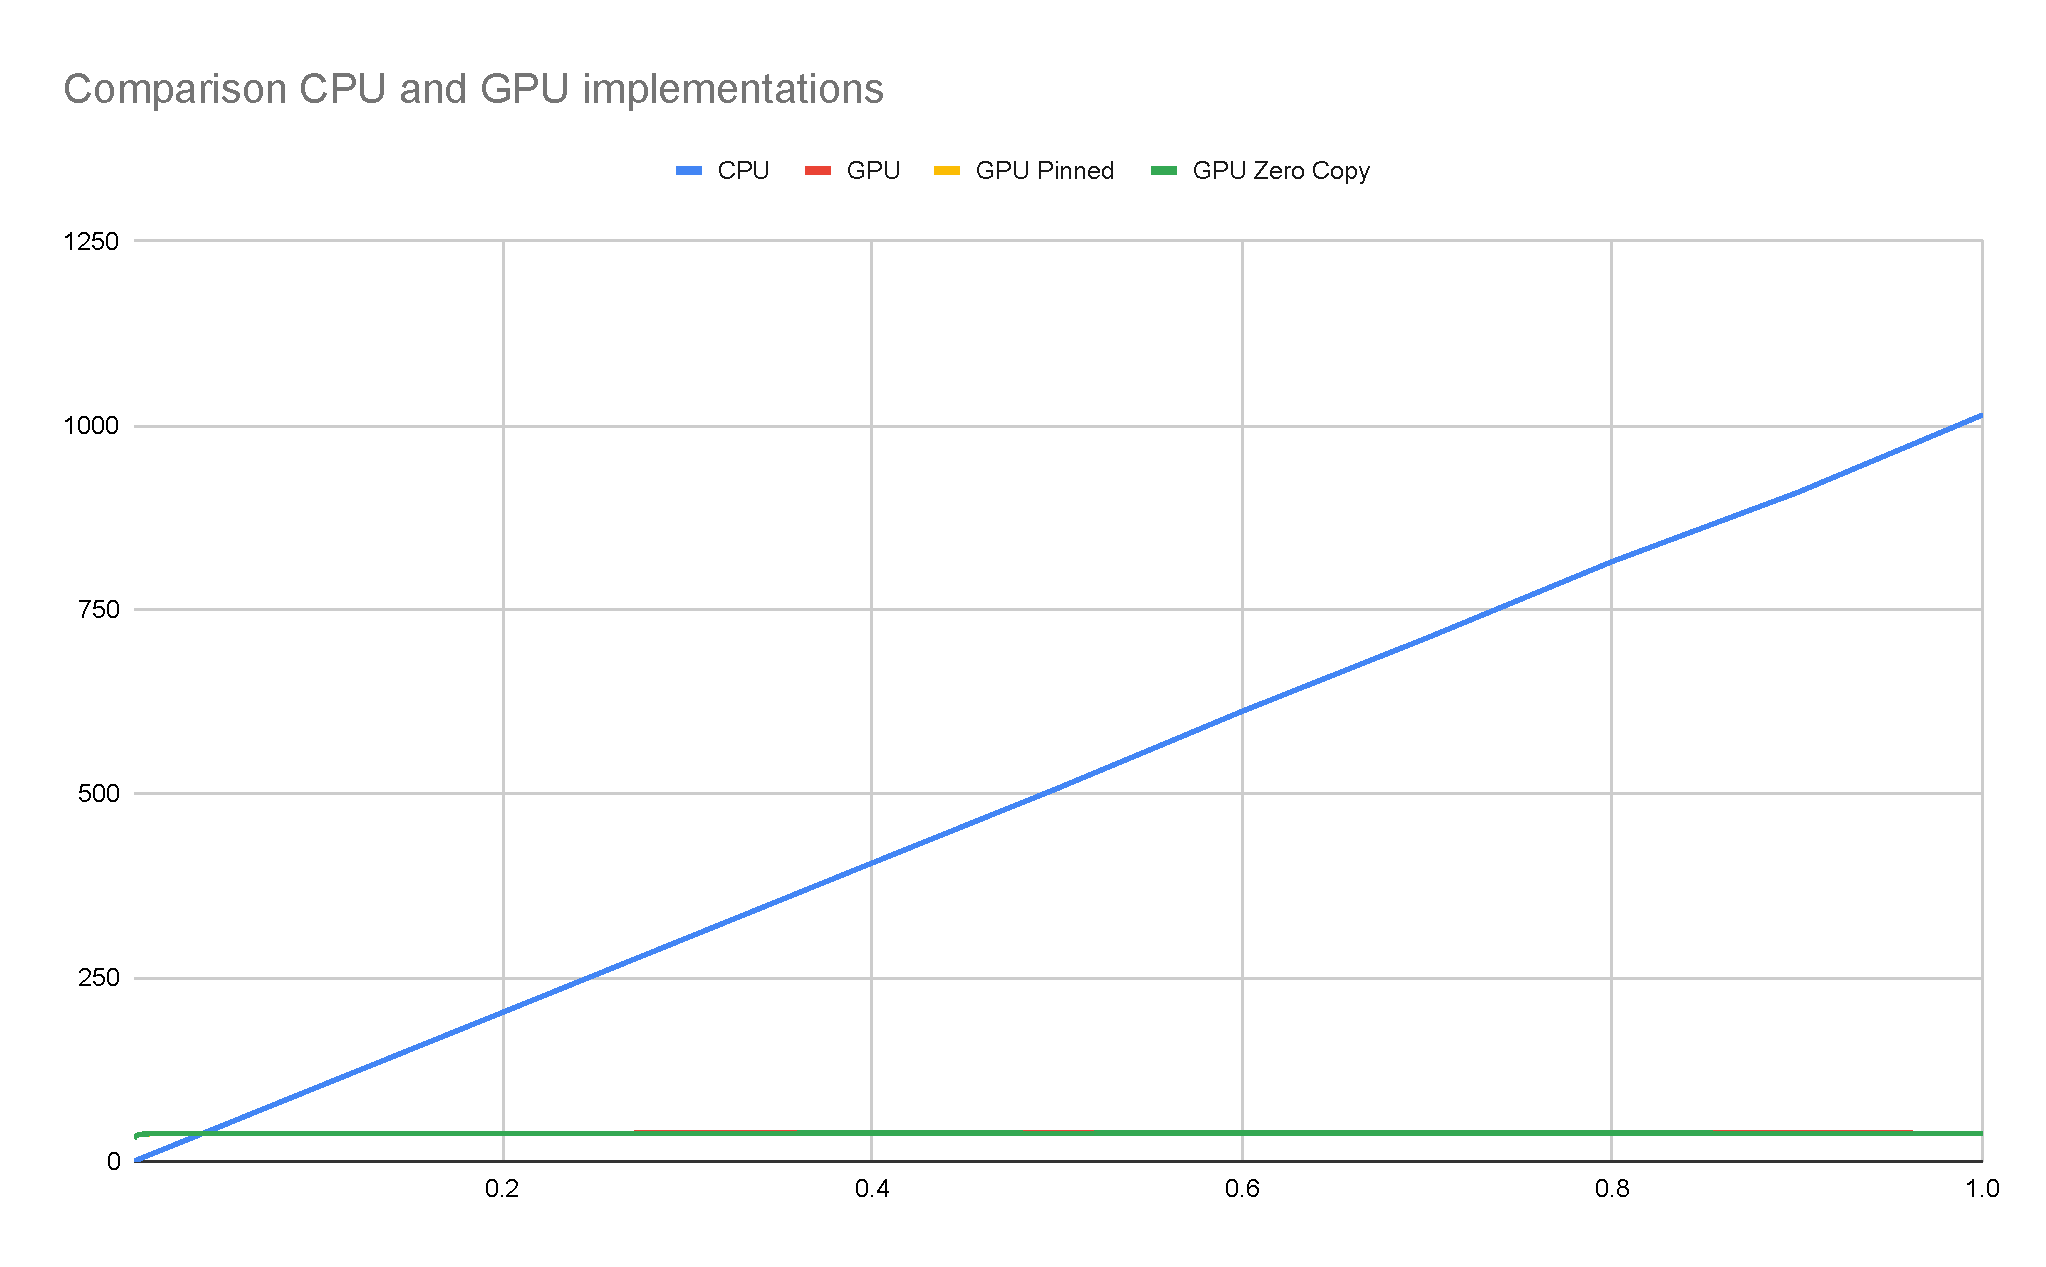
\includegraphics[width=\linewidth]{img/dense_representation/comparison_impl.pdf}
    	\caption{Comparison of dense matrix CPU and GPU implementations}
    	\label{fig:dense_matrix_impl_comparison}
    \end{minipage}%
    \begin{minipage}{.5\textwidth}
    	\centering
    	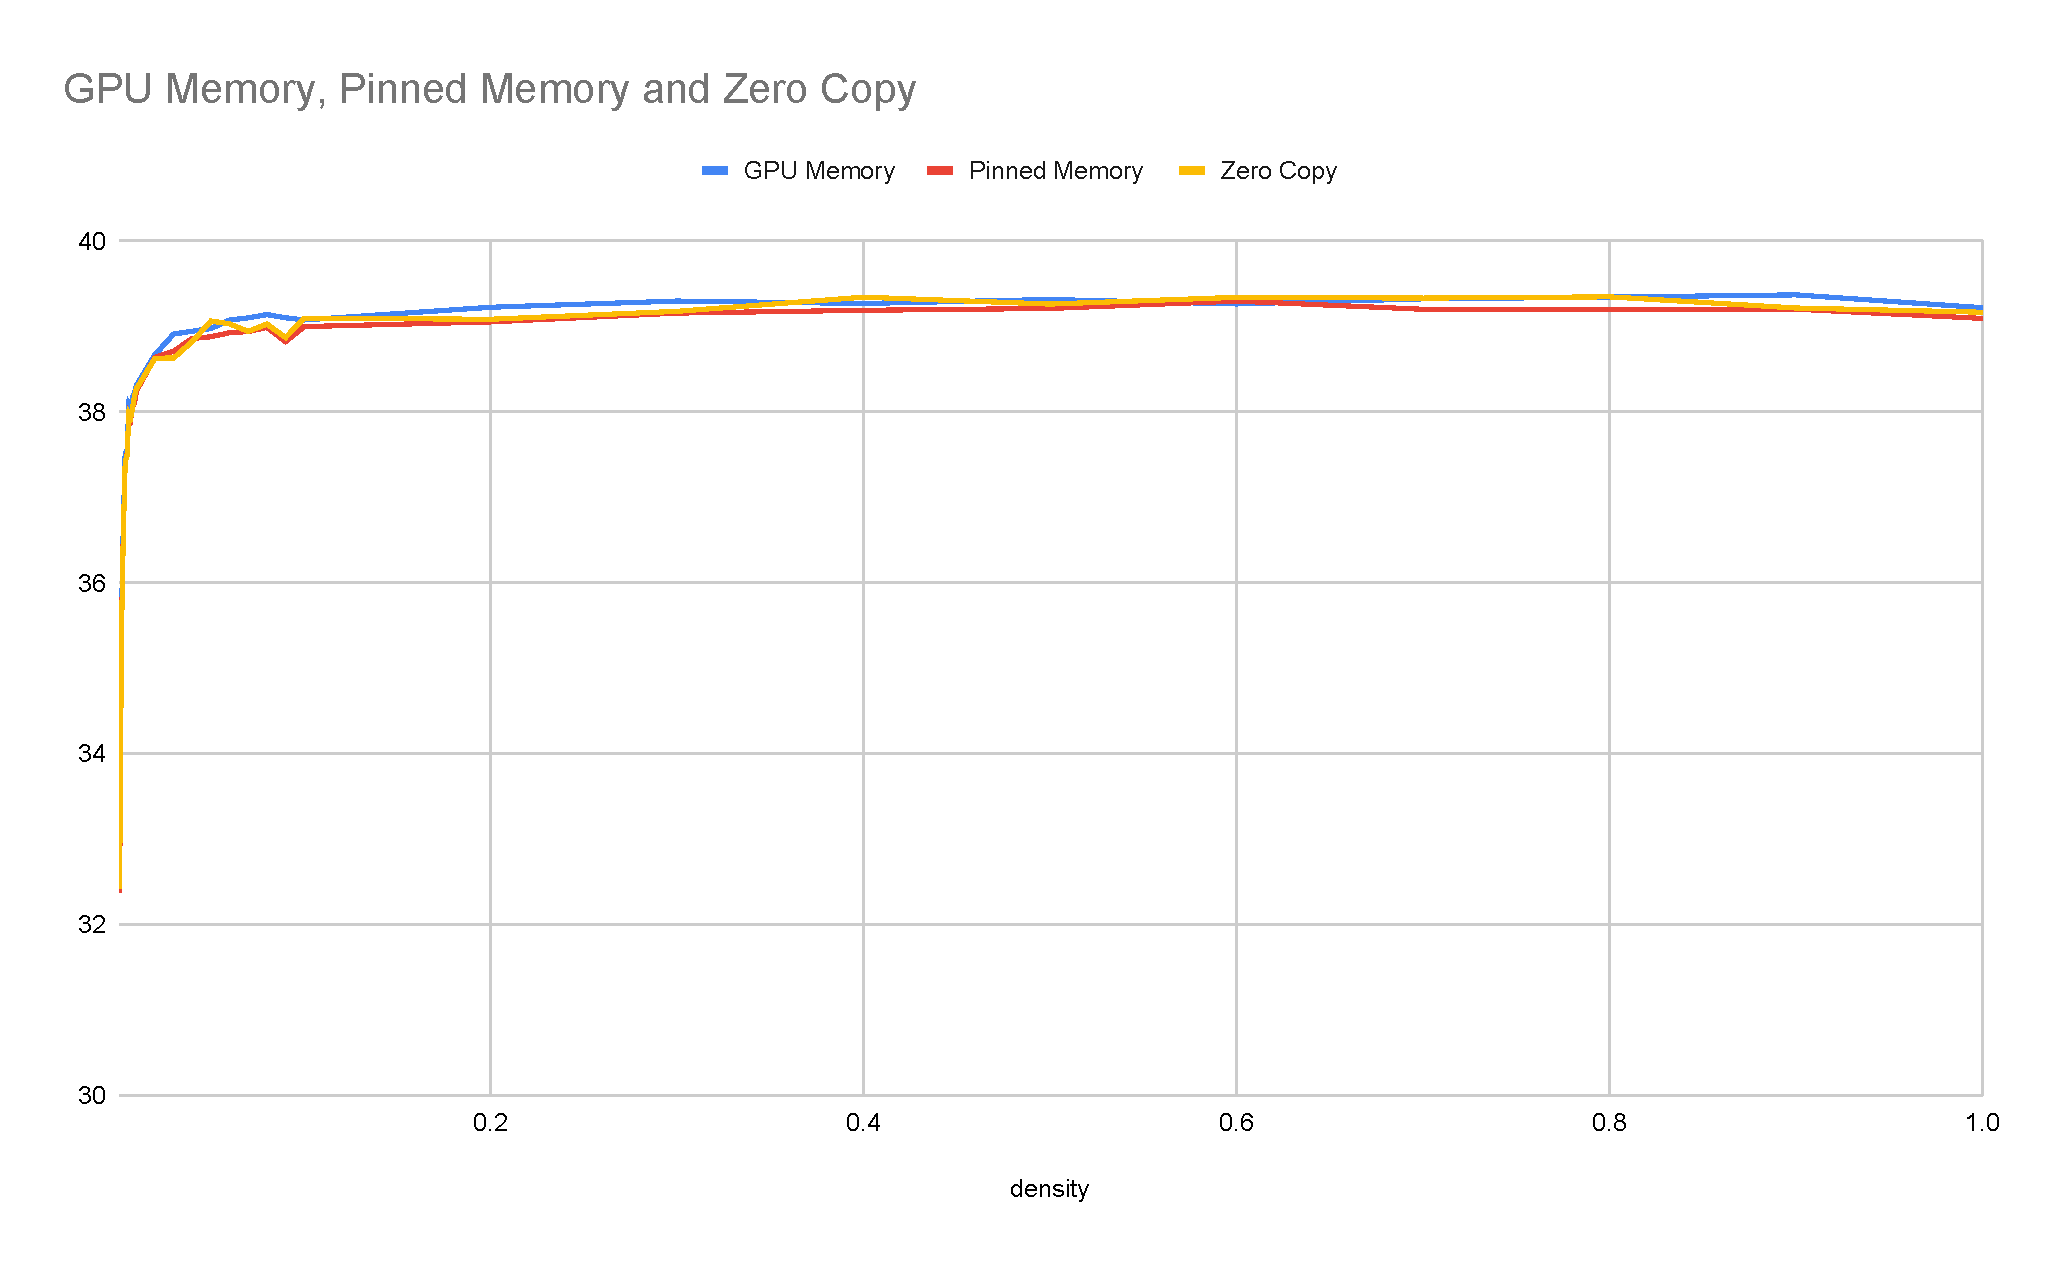
\includegraphics[width=\linewidth]{img/dense_representation/memoyr_comparison.pdf}
    	\caption{Comparison of memory types}
    	\label{fig:dense_matrix_memory_comparison}
    \end{minipage}
\end{figure}

\subsubsection{Evaluation}

In general this algorithm performs quite bad in sparse graphs, where the CPU profits from less comparisons required to be executed. When the graphs get denser, the GPU implementation takes over the lead, as it has the benefit of being able to execute many comparisons in parallel. 

\subsection{Thrust}
%% TODO @manuel


\subsubsection{Input format}
This implimentation uses the same input format already presented in Section~\ref{dense_graph_input_format}.

\subsubsection{Algorithm}

In this algorithm the idea was to treat the calculation of connected components as iterative matrix-like fix-point computation. As the weights can be disregarded for this algorithm they are overwritten in the process.

First off a pre-processing step is taken, which sets all non-zero values of the matrix to their respective column number.

\begin{center}
\begin{tikzpicture}[scale=.7]
  \tikzset{every loop/.style={}}%removes arrow head from all loops.
\node (1) at (2,4) {1};
\node (2) at (4,2) {2};
\node (3) at (3,0) {3};
\node (4) at (1,0) {4};
\node (5) at (0,2) {5};
\draw (1) -- (3);
\path (2) edge[loop] (2);
\draw (2) -- (4);
\draw (4) -- (5);
\end{tikzpicture}
\hfil
\begin{TAB}(e,0.5cm,0.5cm){|c:c:c:c:c|c}{c|c:c:c:c:c|}
    \textbf{1}&\textbf{2}&\textbf{3}&\textbf{4}&\textbf{5}&$\downarrow$\\
    0&0&\textbf{3}&0&0&\\
    0&\textbf{2}&0&\textbf{4}&0&\\
    \textbf{1}&0&0&0&0&\\
    0&\textbf{2}&0&0&\textbf{5}&\\
    0&0&0&\textbf{4}&0&\\
\end{TAB}
\end{center}

Then the first step of the iterative process is taken, by calculating the maximum value per row. This vector is then pivoted and again applied to the non-zero values of the columns, whereby the value is only overridden if it was smaller.

\begin{center}
\begin{TAB}(e,0.5cm,0.5cm){|c:c:c:c:c|c}{c|c:c:c:c:c|}
    &&&&&$\rightarrow$\\
    0&0&3&0&0&\textbf{3}\\
    0&2&0&4&0&\textbf{4}\\
    1&0&0&0&0&\textbf{1}\\
    0&2&0&0&5&\textbf{5}\\
    0&0&0&4&0&\textbf{4}\\
\end{TAB}
\end{center}

This is repeated, until the vector of maximum row values is the same as for the previous iteration, in which case the components have been found. Each position in the resulting vector represents the component id that the node belongs to.

\begin{center}
\begin{TAB}(e,0.5cm,0.5cm){|c:c:c:c:c|c}{c|c:c:c:c:c|}
    \textbf{3}&\textbf{4}&\textbf{1}&\textbf{5}&\textbf{4}&$\downarrow$\\
    0&0&3&0&0&\\
    0&\textbf{4}&0&\textbf{5}&0&\\
    \textbf{3}&0&0&0&0&\\
    0&\textbf{4}&0&0&5&\\
    0&0&0&\textbf{5}&0&\\
\end{TAB}
\hfil
\begin{TAB}(e,0.5cm,0.5cm){|c:c:c:c:c|c}{c|c:c:c:c:c|}
    &&&&&$\rightarrow$\\
    0&0&3&0&0&3\\
    0&4&0&5&0&\textbf{5}\\
    3&0&0&0&0&\textbf{3}\\
    0&4&0&0&5&5\\
    0&0&0&5&0&\textbf{5}\\
\end{TAB}
\hfil
\begin{TAB}(e,0.5cm,0.5cm){|c:c:c:c:c|c}{c|c:c:c:c:c|}
    3&\textbf{5}&\textbf{3}&5&\textbf{5}&$\downarrow$\\
    0&0&3&0&0&\\
    0&\textbf{5}&0&5&0&\\
    3&0&0&0&0&\\
    0&\textbf{5}&0&0&5&\\
    0&0&0&5&0&\\
\end{TAB}
\hfil
\begin{TAB}(e,0.5cm,0.5cm){|c:c:c:c:c|c}{c|c:c:c:c:c|}
    &&&&&$\rightarrow$\\
    0&0&3&0&0&3\\
    0&5&0&5&0&5\\
    3&0&0&0&0&3\\
    0&5&0&0&5&5\\
    0&0&0&5&0&5\\
\end{TAB}
\end{center}

This algorithm has been implemented using thrust transform iterators, gather and transform, which automatically manage the computations as well as the memory accesses. Therefore there is only one variant of this algorithm.

\subsubsection{Evaluation} \label{thrust_evaluation}

\begin{figure}[!h]
    \centering
    \begin{minipage}{.5\textwidth}
    	\centering
    	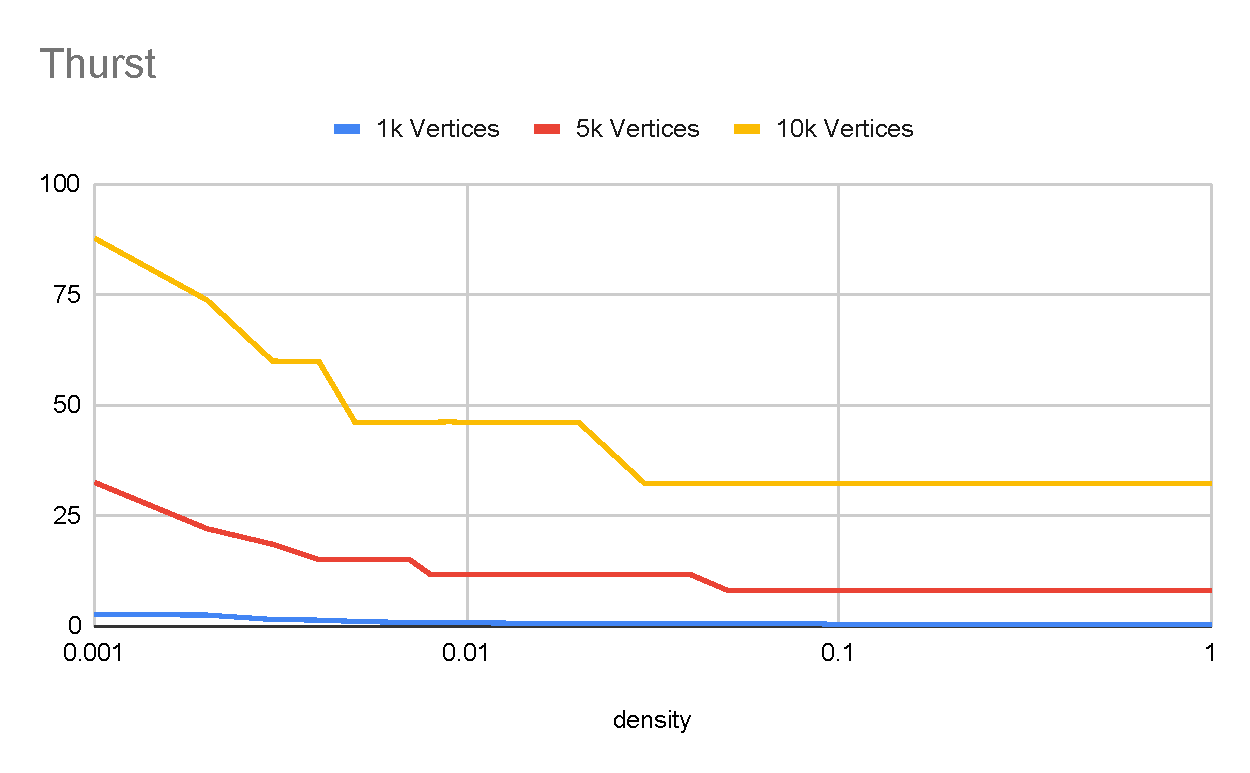
\includegraphics[width=\linewidth]{img/thrust/nodes.pdf}
    	\caption{Comparison different node counts}
    	\label{fig:thrust_node_comparisons}
    \end{minipage}%
    \begin{minipage}{.5\textwidth}
    	\centering
    	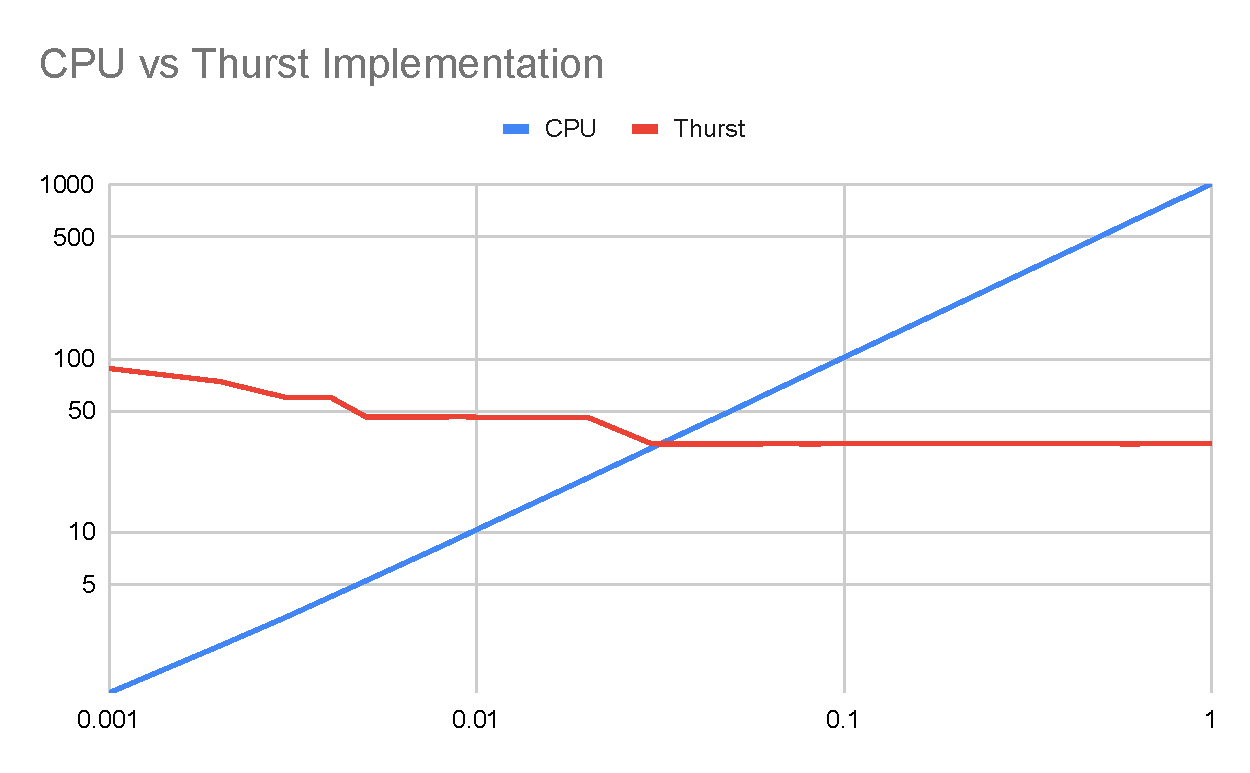
\includegraphics[width=\linewidth]{img/thrust/cpu.pdf}
    	\caption{Comparison to CPU algorithm}
    	\label{fig:thrust_cpu_comparison}
    \end{minipage}
\end{figure}

As can be seen in \ref{fig:thrust_node_comparisons}, the performance of the algorithm increases as the density rises. This is due to the fact, that the algorithm needs fewer iterations to find the fix-point, as all connections to a node are checked at once. This is especially noticeable in \ref{fig:thrust_cpu_comparison}, where it can be seen that the algorithm strongly outperforms the CPU implementation at higher densities.

\newpage
\section{Comparison}\label{sec:compare}
In Figure~\ref{fig:impl_comparison} the run-time measurements of the single implementations are depicted. For the GPU implementations, we used the devices memory and each tested graph consists of 10,000. On the x-axis the graph density is depicted in a logarithmic scale. The test points were scattered in a logarithmic fashion to reduce the run-time required for our tests. The y-axis the shows the run-time in seconds.

The graph problem of finding connected components is commonly known to be hard to parallelize and doesn't benefit greatly from adding more threads to solve such a problem. Finding connected components requires a lot of communication between the single threads and optimized data structures are required. The sparse graph representation uses pointers and lists which are beneficial an play out the strengths of the CPU by having a higher clock and being faster when accessing random memory addresses. For less dense graphs this approach can be used on the GPU, but the memory architecture profits from aligned memory access, which hurts the algorithm when considering denser graphs. This can be seen in Figure~\ref{fig:impl_comparison} as the lines for the sparse representation significantly grow at a graph density of 0.2. In contrast when switching to the dense matrix representation, the required memory is aligned and the GPU has optimized access, but it requires a lot more iterations over the data structure. In Figure~\ref{fig:impl_comparison} the dense matrix representation has a fairly constant execution time, mainly dependent on the graph size, but this run-time is way higher in contrast to the CPU. Computing the dense matrix representation via the Thrust algorithm even exhibits performance uplifts with higher densities, as explained in \ref{thrust_evaluation}.

\begin{figure}
	\centering
	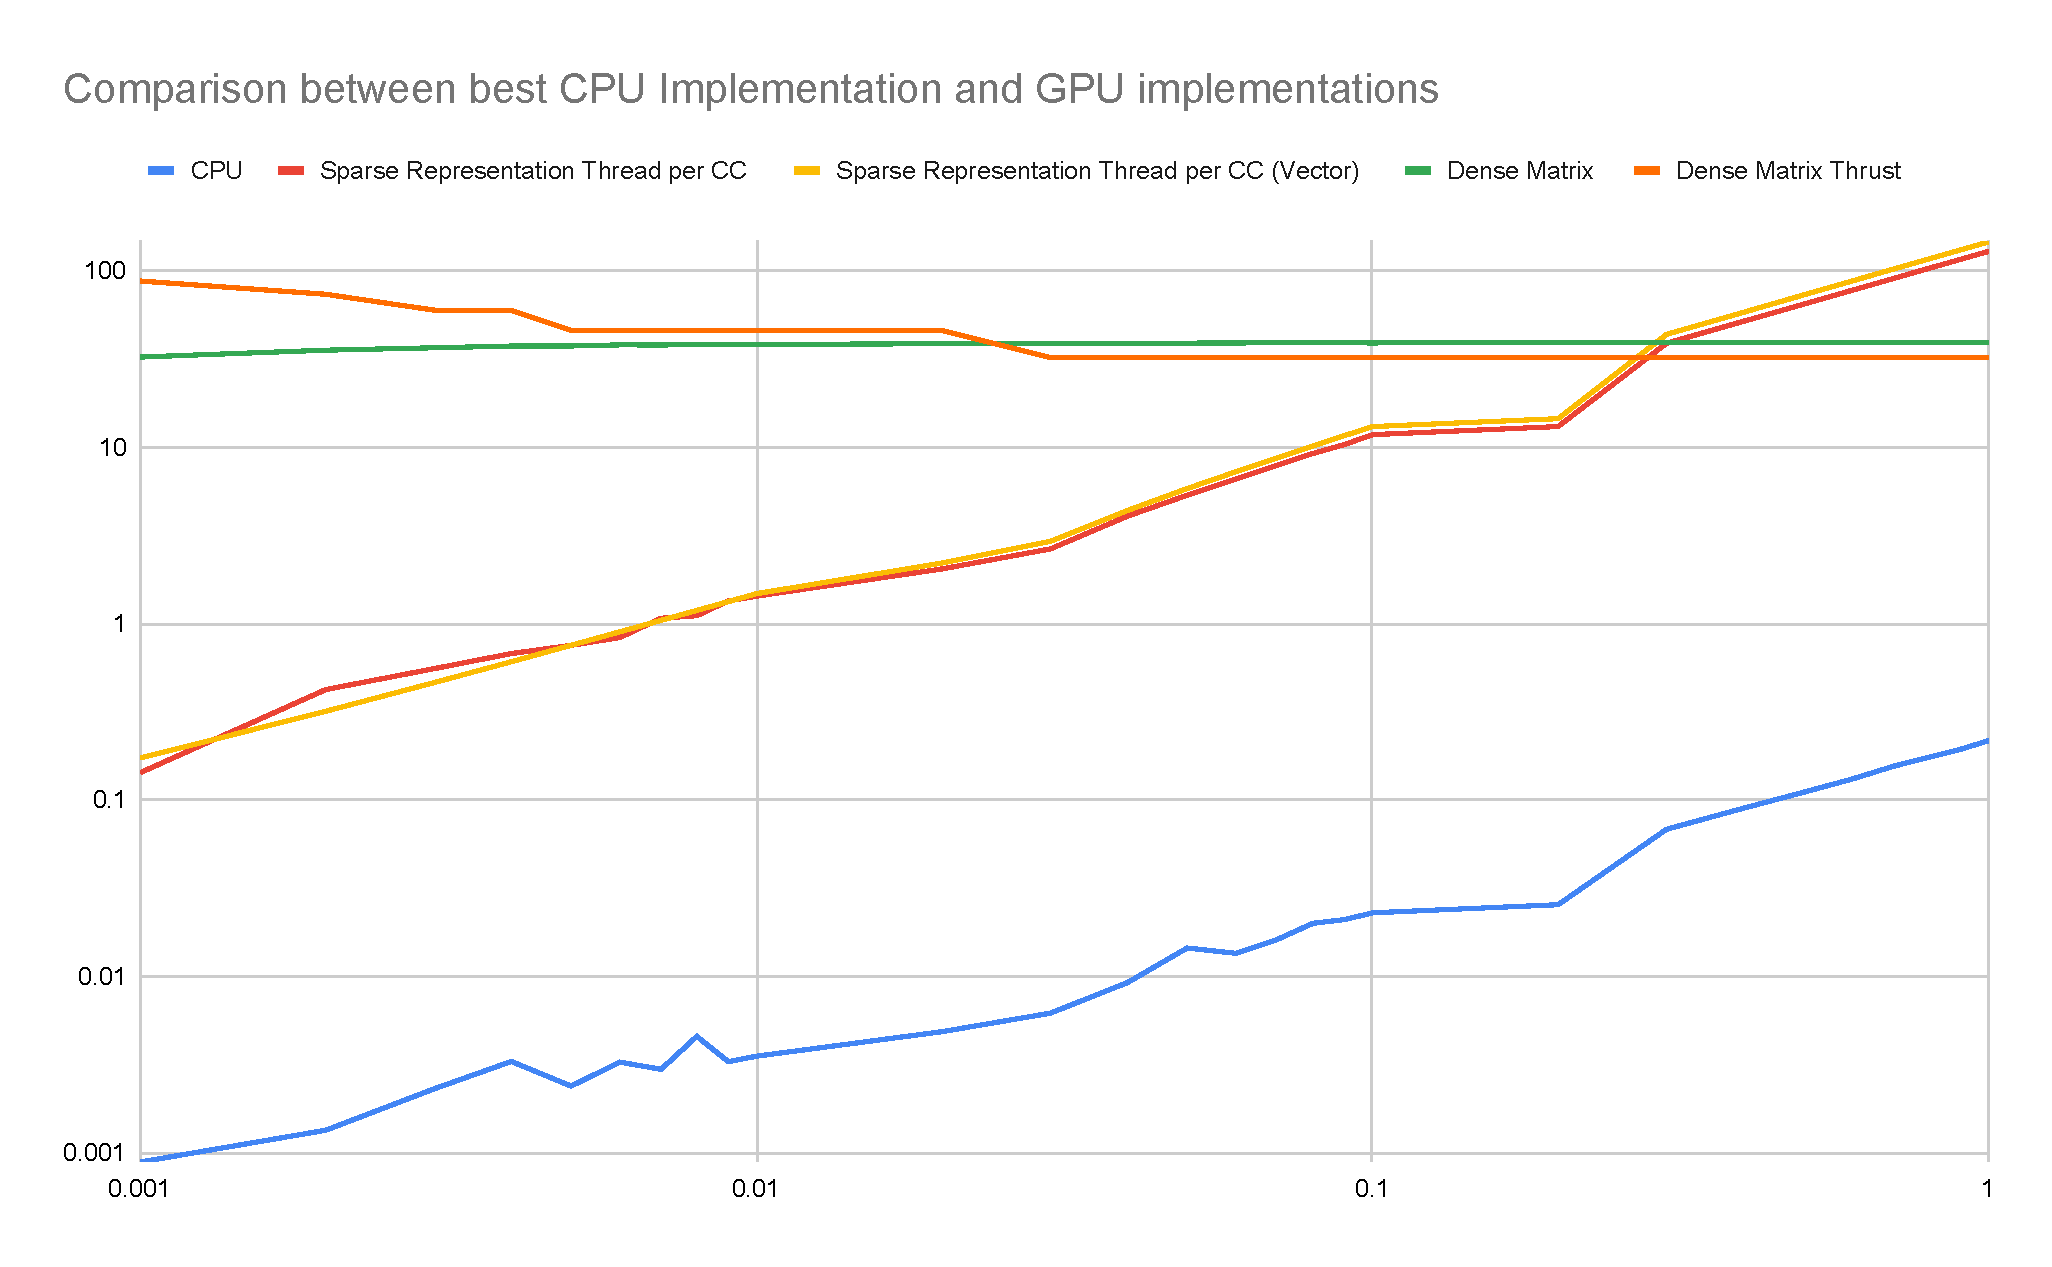
\includegraphics[width=\linewidth]{img/comparison_all.pdf}
	\caption{Comparison of the best CPU implementation and the GPU implementations}
	\label{fig:impl_comparison}
\end{figure}

\end{document} 
